
\documentclass[]{article}
%\documentclass[journal,10pt,draftclsnofoot,onecolumn]{IEEEtran}
%\usepackage{graphics,multirow,amsmath,amssymb,textcomp,subfigure,multirow,xspace,arydshln,cite}

\usepackage[]{graphicx}   % para manejar graficos

\usepackage[space]{grffile} % para manejar graficos

\usepackage{caption}

\usepackage{enumerate}    % para hacer listas numeradas

\usepackage{amsmath}        % no se..

\usepackage{amsfonts}     % no se..

\usepackage{authblk}    % para definir las afiliaciones de cada autor

\usepackage{layout}     % no se..

\usepackage{biblatex}     % para manejar la bibliografia / referencias

\usepackage{lipsum}     % para generar texto random

\usepackage{multicol}   % para usar dos columnas

\usepackage{palatino}   % para que la fuente sea palatino

\usepackage[utf8]{inputenc} % para poder usar tildes

\usepackage[spanish]{babel} % para escribir en español

\usepackage[sc,big,raggedright,bf]{titlesec} % para definir el formato del header de cada seccion.

\usepackage[font=small]{caption} % para que la fuente de un epigrafe no tenga el mismo tamaño que el cuerpo del texto

\usepackage{geometry}
 \geometry{
 a4paper,
 textwidth={17cm},
 textheight={23cm},
 left={2cm},
 top={2.5cm},
 }

\setlength{\columnsep}{1cm} % para que la separacion entre columnas sea de 1 cm

\graphicspath {{imagenes/}}

\defbibheading{bibliography}{\section{\refname}} % para que bibtex no imponga su header cuando uso \printbibliography, y que se use el de babel

\addbibresource{bibliografia.bib} % para importar el archivo .bib

\title{\textbf{\LARGE{\textsf{TITÚLO DEL PAPER O INFORME}}}}
 % defino el titulo del Paper

\date{} % lo pongo vacio para que no aparezca abajo del abstract

\usepackage{fancyhdr}

%%%%%%%%%%%%%%%%%%%%%%%%%%%%%%%%%%%%%%%%%%%%%%%%%%%%%%%%%%%%%%%%%%%%%%%%%%%%%%%%%
% http://www-h.eng.cam.ac.uk/help/tpl/textprocessing/multicol_hint.html
\makeatletter           % esto lo uso para poder definir figuras
\newenvironment{tablehere}    % esto lo uso para poder definir figuras
  {\def\@captype{table}}    % esto lo uso para poder definir figuras

  {}              % esto lo uso para poder definir figuras
                  % esto lo uso para poder definir figuras
\newenvironment{figurehere}   % esto lo uso para poder definir figuras
  {\def\@captype{figure}}   % esto lo uso para poder definir figuras
  {\par\medskip}
  {}              % esto lo uso para poder definir figuras
\makeatother          % esto lo uso para poder definir figuras
%%%%%%%%%%%%%%%%%%%%%%%%%%%%%%%%%%%%%%%%%%%%%%%%%%%%%%%%%%%%%%%%%%%%%%%%%%%%%%%%%

%%%%%%%%%%%%%%%%%%%%%%%%%%%%%%%%%%%%%%%%%%%%%%%%%%%%%%%%%%%%%%%%%%%%%%%%%%%%%%%%%
%               ACA EMPIEZA EL DOCUMENTO                            %
%%%%%%%%%%%%%%%%%%%%%%%%%%%%%%%%%%%%%%%%%%%%%%%%%%%%%%%%%%%%%%%%%%%%%%%%%%%%%%%%%


\begin{document} % empieza el documentoo


\renewcommand{\headrulewidth}{0pt} % para que no haya linea decorativa en el header.


\author[1]{Nombre y Apellido} % defino el autor
\affil[1]{Universidad Nacional de Tres De Febrero, Buenos Aires, Argentina \newline \texttt{email@delautor.com}} % afiliacion del autor


\begin{minipage}[h]{\textwidth} % uso el entorno minipage para que el abstract este en la misma pagina que el titulo
    \maketitle
    \thispagestyle{fancy}
    \fancyhf{}
    \rhead{Fecha de entrega}
    \lhead{Materia/Congreso}
    \cfoot{\thepage}

\end{minipage}


\begin{abstract}

\textit{\lipsum[1]}
\end{abstract}

\begin{multicols}{2}
\section{Introducción}
\lipsum[2]
\section{Trabajos Previos}
\lipsum[3]
\section{Conceptos y términos básicos}
\lipsum[4]
\section{Arreglo experimental}
\lipsum[5]
\
Para esta medición, se puede utilizar equipamiento simple y obtener resultados fiables.

El instrumental utilizado es el siguiente:
\begin{itemize}
  \item Un Osciloscopio Tektronix 2049b
  \item Un generador de señales Nike
  \item Un Ford fiesta
\end{itemize}
\subsection{Método 1}
\lipsum[6]
Al variar $\omega$ entre $0$ y $2 \pi$, se obtiene la figura \ref{fig:circulo}:

\begin{figurehere}
 \centering
 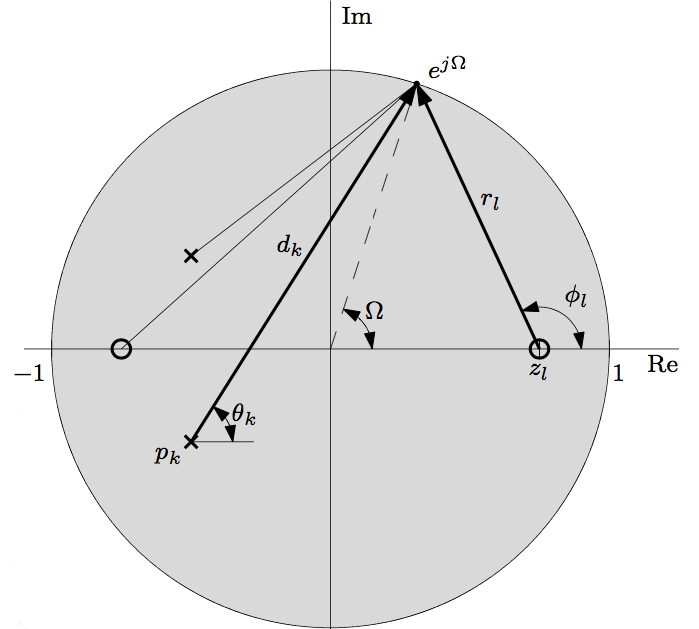
\includegraphics[width=\linewidth]{lathi}
 \captionof{figure}{Los polos y los ceros determinan $H(z)$}
 \label{fig:circulo}
\end{figurehere}

\subsection{Método 2} % SI APLICA
\lipsum[7]
Se puede encontrar una demostración detallada en \cite{Sh:575} , \cite{Sh:572}.
\subsection{Método 3} % SI APLICA
\
\lipsum[8] En \cite{webster} se puede ver que:

\begin{equation}
 e^{ \ j  \pi} = -1
 \label{euler}
\end{equation}
La ecuancion \ref{euler} es conocida como la identidad de Euler.

\section{Resultados}

La tabla \ref{Vgs} muestra la relacion entre las dos variables en cuestión:

\begin{tablehere}
\begin{center}
\begin{tabular}{|c|c|c|c|}
\hline
$V_{GS}$ [V] & $I_{D}$ [A] & Temperatura [$C^{o}$] & $\frac{V_{GS}}{I_D}$ [$\Omega$] \\
\hline
col1 & col2 & col3 & col4 \\

col1 & col2 & col3 & col4 \\

col1 & col2 & col3 & col4 \\
\hline
\end{tabular}
\caption{Variación de $\frac{V_{GS}}{I_D}$}
\label{Vgs}
\end{center}
\end{tablehere}

\lipsum[1]


\section{Análisis de resultados}
\lipsum[1]
\section{Conclusión}
\lipsum[1]

\printbibliography
\end{multicols}



\end{document}
